%; whizzy document
% latex beamer presentation.

%     Copyright (C) 2007 Junichi Uekawa

%     This program is free software; you can redistribute it and/or modify
%     it under the terms of the GNU General Public License as published by
%     the Free Software Foundation; either version 2 of the License, or
%     (at your option) any later version.

%     This program is distributed in the hope that it will be useful,
%     but WITHOUT ANY WARRANTY; without even the implied warranty of
%     MERCHANTABILITY or FITNESS FOR A PARTICULAR PURPOSE.  See the
%     GNU General Public License for more details.

%     You should have received a copy of the GNU General Public License
%     along with this program; if not, write to the Free Software
%     Foundation, Inc., 51 Franklin St, Fifth Floor, Boston, MA  02110-1301 USA

\documentclass[dvipdfm,12pt]{beamer}
%\usetheme{}

%  preview (shell-command (concat "xpdf " (replace-regexp-in-string "tex$" "pdf"(buffer-file-name)) "&"))
%  presentation (shell-command (concat "xpdf -fullscreen " (replace-regexp-in-string "tex$" "pdf"(buffer-file-name)) "&"))
%  presentation-evince (shell-command (concat "evince " (replace-regexp-in-string "tex$" "pdf"(buffer-file-name)) "&"))

\title{what's happening with pbuilder?}
\subtitle{Debian Conference 2007}
\author{dancer@debian.org}
\date{June 2007}
\logo{
\includegraphics[width=8cm]{openlogo-light.eps}}

\begin{document}
\frame{\titlepage{}}


\begin{frame}{Who am I?}
\begin{itemize}
 \item Junichi Uekawa, dancer@debian.org
 \item Lives in Japan, Debian JP Project Leader for 2007
 \item Debian Developer since 2000
 \item Interests: Audio-processing related tools, and 
       Debian quality maintenance related tools,
       Japanese localization, shared library packaging, 
       and more recently, Debian/MacBook related.
\end{itemize}
\end{frame}
 
\begin{frame}{pbuilder basics}
\includegraphics[height=0.7\vsize]{pbuildercycle.eps}
\end{frame}

\begin{frame}{pbuilder basics ...}
\begin{tabular}{|l|p{8em}|p{8em}|}
\hline
operation & frequence & meaning \\
\hline
create & once in initial run & create base filesystem \\
update & twice a day (according to unstable updates) & 
 revise base filesystem \\
build & for each package build & build Debian package inside chroot \\
\hline
\end{tabular}
\end{frame}

\begin{frame}[containsverbatim]{pbuilder create}
\begin{verbatim}
# pbuilder create
Distribution is sid.
Building the build environment
 -> running debootstrap
/usr/sbin/debootstrap
I: Retrieving Release
I: Retrieving Packages
I: Validating Packages
	.
	.
\end{verbatim}
\end{frame}


\begin{frame}[containsverbatim]{pbuilder update}
\begin{verbatim}
# pbuilder update
W: /home/dancer/.pbuilderrc does not exist
Building the build Environment
 -> extracting base tarball [/var/cache/pbuilder/base.tgz]
	.
	.
\end{verbatim}
\end{frame}

\begin{frame}[containsverbatim]{pbuilder build}
\begin{verbatim}
# pbuilder build dsh_*.dsc
I: using fakeroot in build.
Current time: Sat Jan 20 12:03:34 JST 2007
pbuilder-time-stamp: 1169262214
Building the build Environment
 -> extracting base tarball [/home/dancer/DEBIAN/pbuilder/pbuilder/testsuite/tmp.FeeAX18779/testimage]
 -> creating local configuration
	.
	.
\end{verbatim}
\end{frame}

\begin{frame}{pbuilder basics ...}
\begin{minipage}{0.4\hsize}
 How do you maintain your package today?
\end{minipage}
\begin{minipage}{0.5\hsize}
  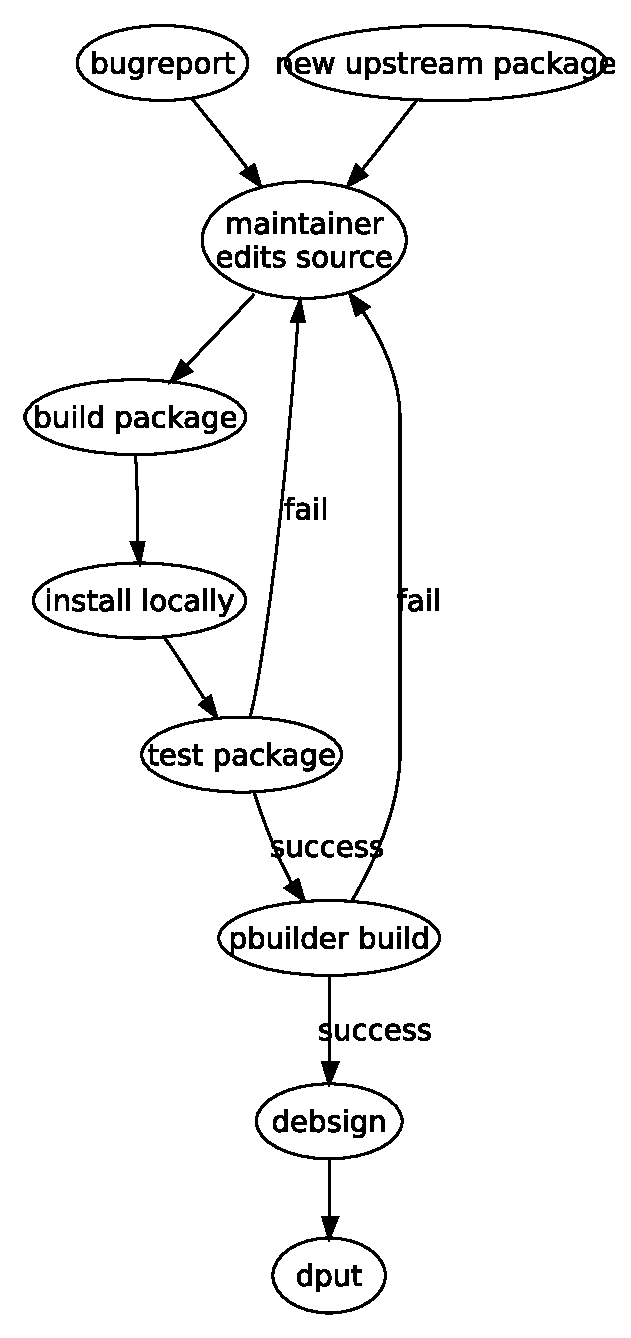
\includegraphics[height=0.9\vsize]{develcycle.eps}
\end{minipage}
\end{frame}

\begin{frame}[containsverbatim]{Development}

alioth project: \url{http://alioth.debian.org/projects/pbuilder}

\begin{verbatim}
git-clone
  ssh://git.debian.org/git/pbuilder/pbuilder.git
\end{verbatim}
\end{frame}

\begin{frame}{pbuilder backend variations}
\begin{minipage}{0.5\hsize}
 Motivation
\begin{itemize}
 \item limitation in chroot segregation (process space, filesystem)
 \item COW filesystem optimization
\end{itemize}
\end{minipage}\begin{minipage}{0.4\hsize}
  \begin{itemize}
  \item LVM
  \item UML
  \item cowdancer
  \item qemu
 \end{itemize}
\end{minipage}
\end{frame}

\begin{frame}{further ideas}
 \begin{itemize}
  \item install testing
  \item package testing
 \end{itemize}
\end{frame}

\begin{frame}{related tools}
 \begin{itemize}
  \item schroot
  \item piuparts
  \item autopkgtest
 \end{itemize}
\end{frame}

\end{document}
